\section{Реализация}
\subsection{Набор данных}
Мною был выбран датасет MovieLens 1M \cite{voc3}, включающий в себя 1 миллион оценок 4,000 фильмов от 6,000 пользователей.
\subsection{Scikit SurPRISE}
SurPRISE \cite{voc4} -- библиотека на языке Python, которая включает в себя реализацию построения и анализа рекомендательных систем. 
Из этого пакета, был использован метод SVD для построения рекомендательной системы.
\begin{figure}[ht]
  \begin{center}
  \scalebox{0.3}{
     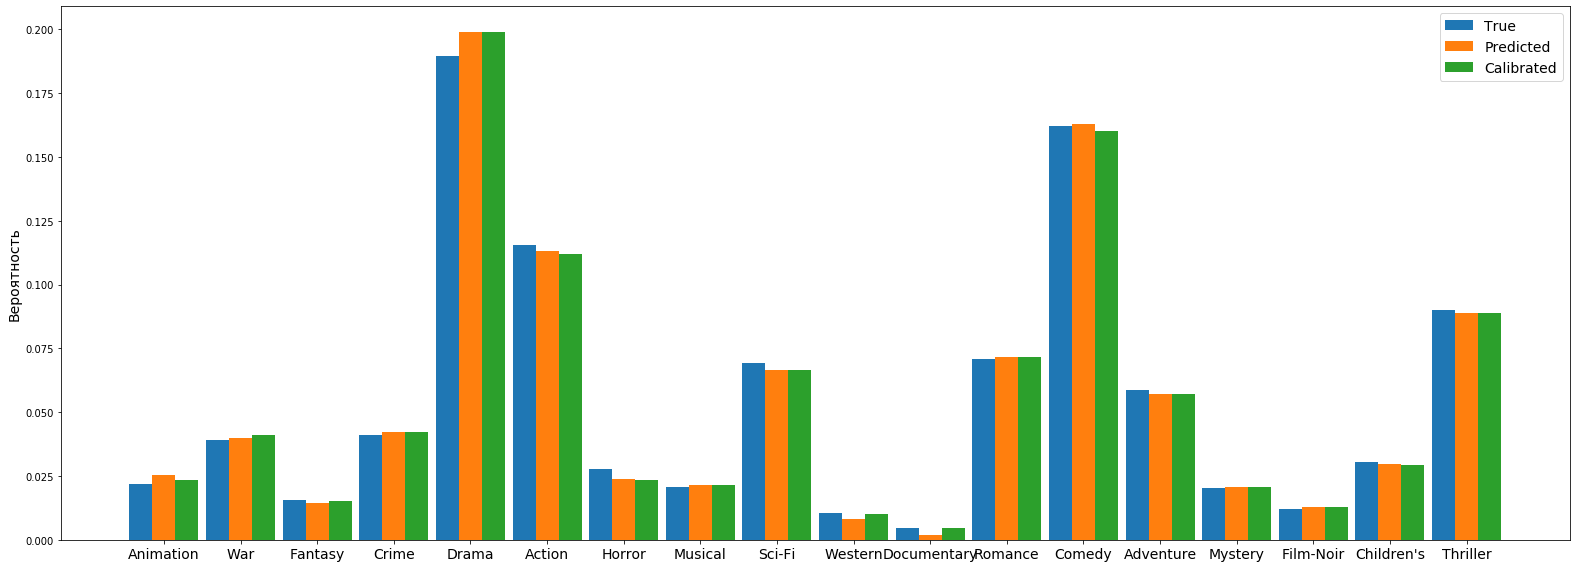
\includegraphics{images/graph.png}
  }
  
  \caption{
  \label{graph-fig}
       Распределение жанров.}
  \end {center}
  \end {figure}


  \subsection{Результаты}
  Получив вектор предсказаний, я построил графики реального, предсказанного и откалиброванного распределения жанров фильмов для всех пользователей, они изображены на рисунке \ref{graph-fig}. 
  Как видно на графике, распределение, полученное рекомендательной системой, плохо отражает такие жанры, как вестерн и документальное кино, а после калибровки распределение стало ближе к реальному. 
  Калибровка была произведена с помощью расстояния Кульбака-Лейблера по формуле (\ref{eq:Calibrated}), с коэффициентом $\lambda=0.2$.
  